\documentclass[12pt]{book}
\usepackage{graphicx}
\usepackage{geometry}
\usepackage{titlesec}
% \usepackage{marginnote}
\usepackage{amsmath}
\usepackage{multicol}


% Set geometry for large margin on the side
\geometry{
    left=1.25in,
    right=3in, % Larger margin for notations on the right
    top=1in,
    bottom=1in
}

% Customize chapter title to place image right after title
\titleformat{\chapter}[display]
  {\normalfont\Large\bfseries} % Change font and style
  {\chaptertitlename\ \thechapter}{20pt}{\Huge} % Change spacing
  [\vspace{1em}\hrule\vspace{1em}] % Line after title

% Begin document
\begin{document}

\tableofcontents

% ###################################################################################################
% Chapter 0 - Presentation
% ###################################################################################################

\chapter{Presentation}

% Chapter-wide image
\begin{center}
    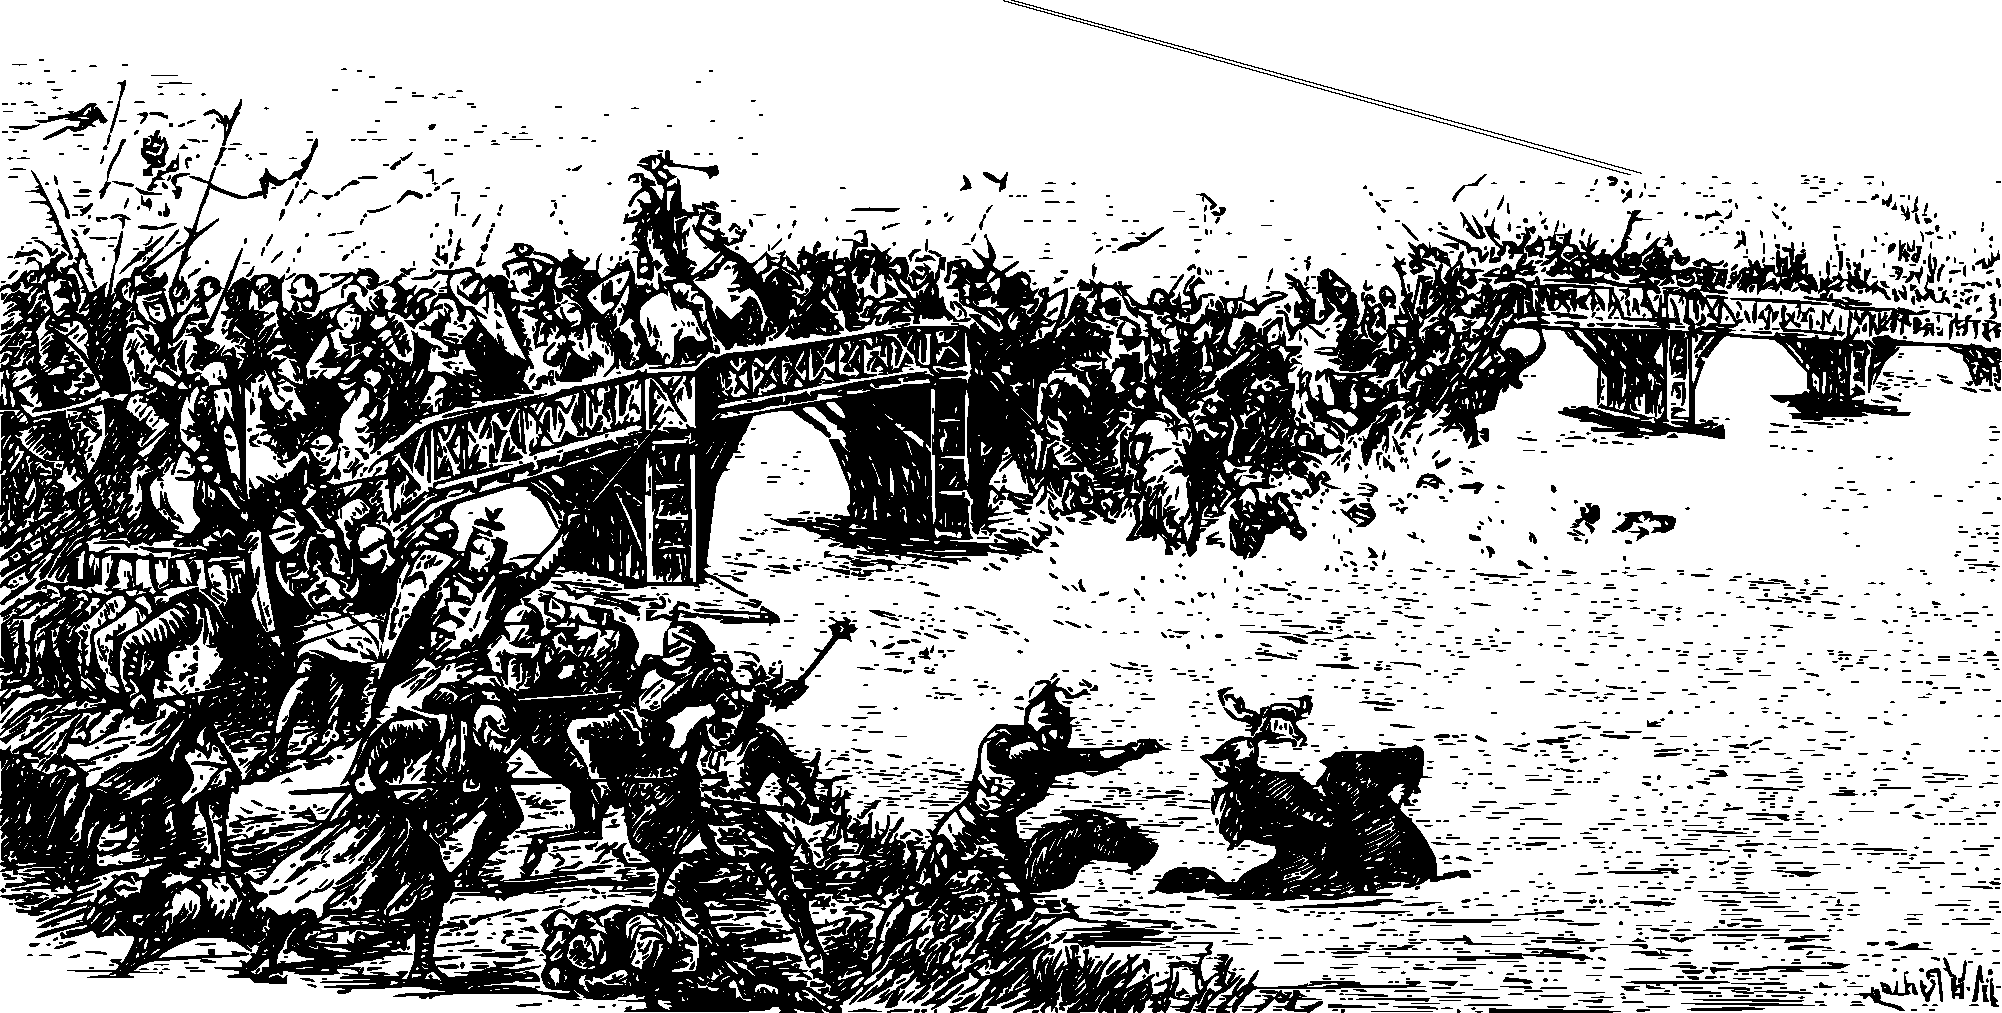
\includegraphics[width=\textwidth]{./images/presentation01.pdf}
\end{center}

% \marginnote{\small \textit{Note: These margins are designed to allow space for important notations and additional context.}}

In the realm of tabletop role-playing games, Eidos stands as a unique and innovative addition to the genre. Rooted in open-source principles, this game is designed to be both immersive and accessible...

The character creation process in Eidos is a deep and engaging experience, allowing players to build their characters from the ground up. With character sheets devoted to personality, religion, physical description, background, clothing, equipment, and skills, players have the tools to create a truly unique and memorable character.

The combat system in Eidos is designed to be immersive and engaging, with mechanics that are designed to create dynamic and exciting combat scenes. The game's mechanics are based on classic combat narratives, and the system strives to be a simulation of combat rather than simply a turn-based dice-rolling game. The standard rules are designed to be played in a pre-modern low-fantasy setting, but the game is easily adaptable to other role-playing scenarios.

This rulebook is divided into six chapters, each of which covers a different aspect of the game. Chapter 1: Character Creation provides a detailed guide to creating your character, including sections on personality, religion, physical description, background, clothing, equipment, and skills. Chapter 2: Combat and Combat Resolution covers the mechanics of combat in Eidos, including basic combat mechanics, ability checks, skills, tactical maneuvering, environmental interaction, morale, reinforcements, ranged combat, unarmed combat, weapon mechanics, grappling, healing, shields and armor, mounted combat, naval combat, aerial combat, siege weapons, traps, stealth, mass combat, and death and dying.

Chapter 3: Survival Mechanics covers the mechanics of survival in Eidos, including food and water requirements, shelter, scavenging, travel, and exploration. Chapter 4: Character Injuries and Health provides a comprehensive guide to character injuries and health, including damage and wound mechanics, healing and recovery, status effects, and advanced injuries and trauma.

\begin{figure}[h]
    \centering
    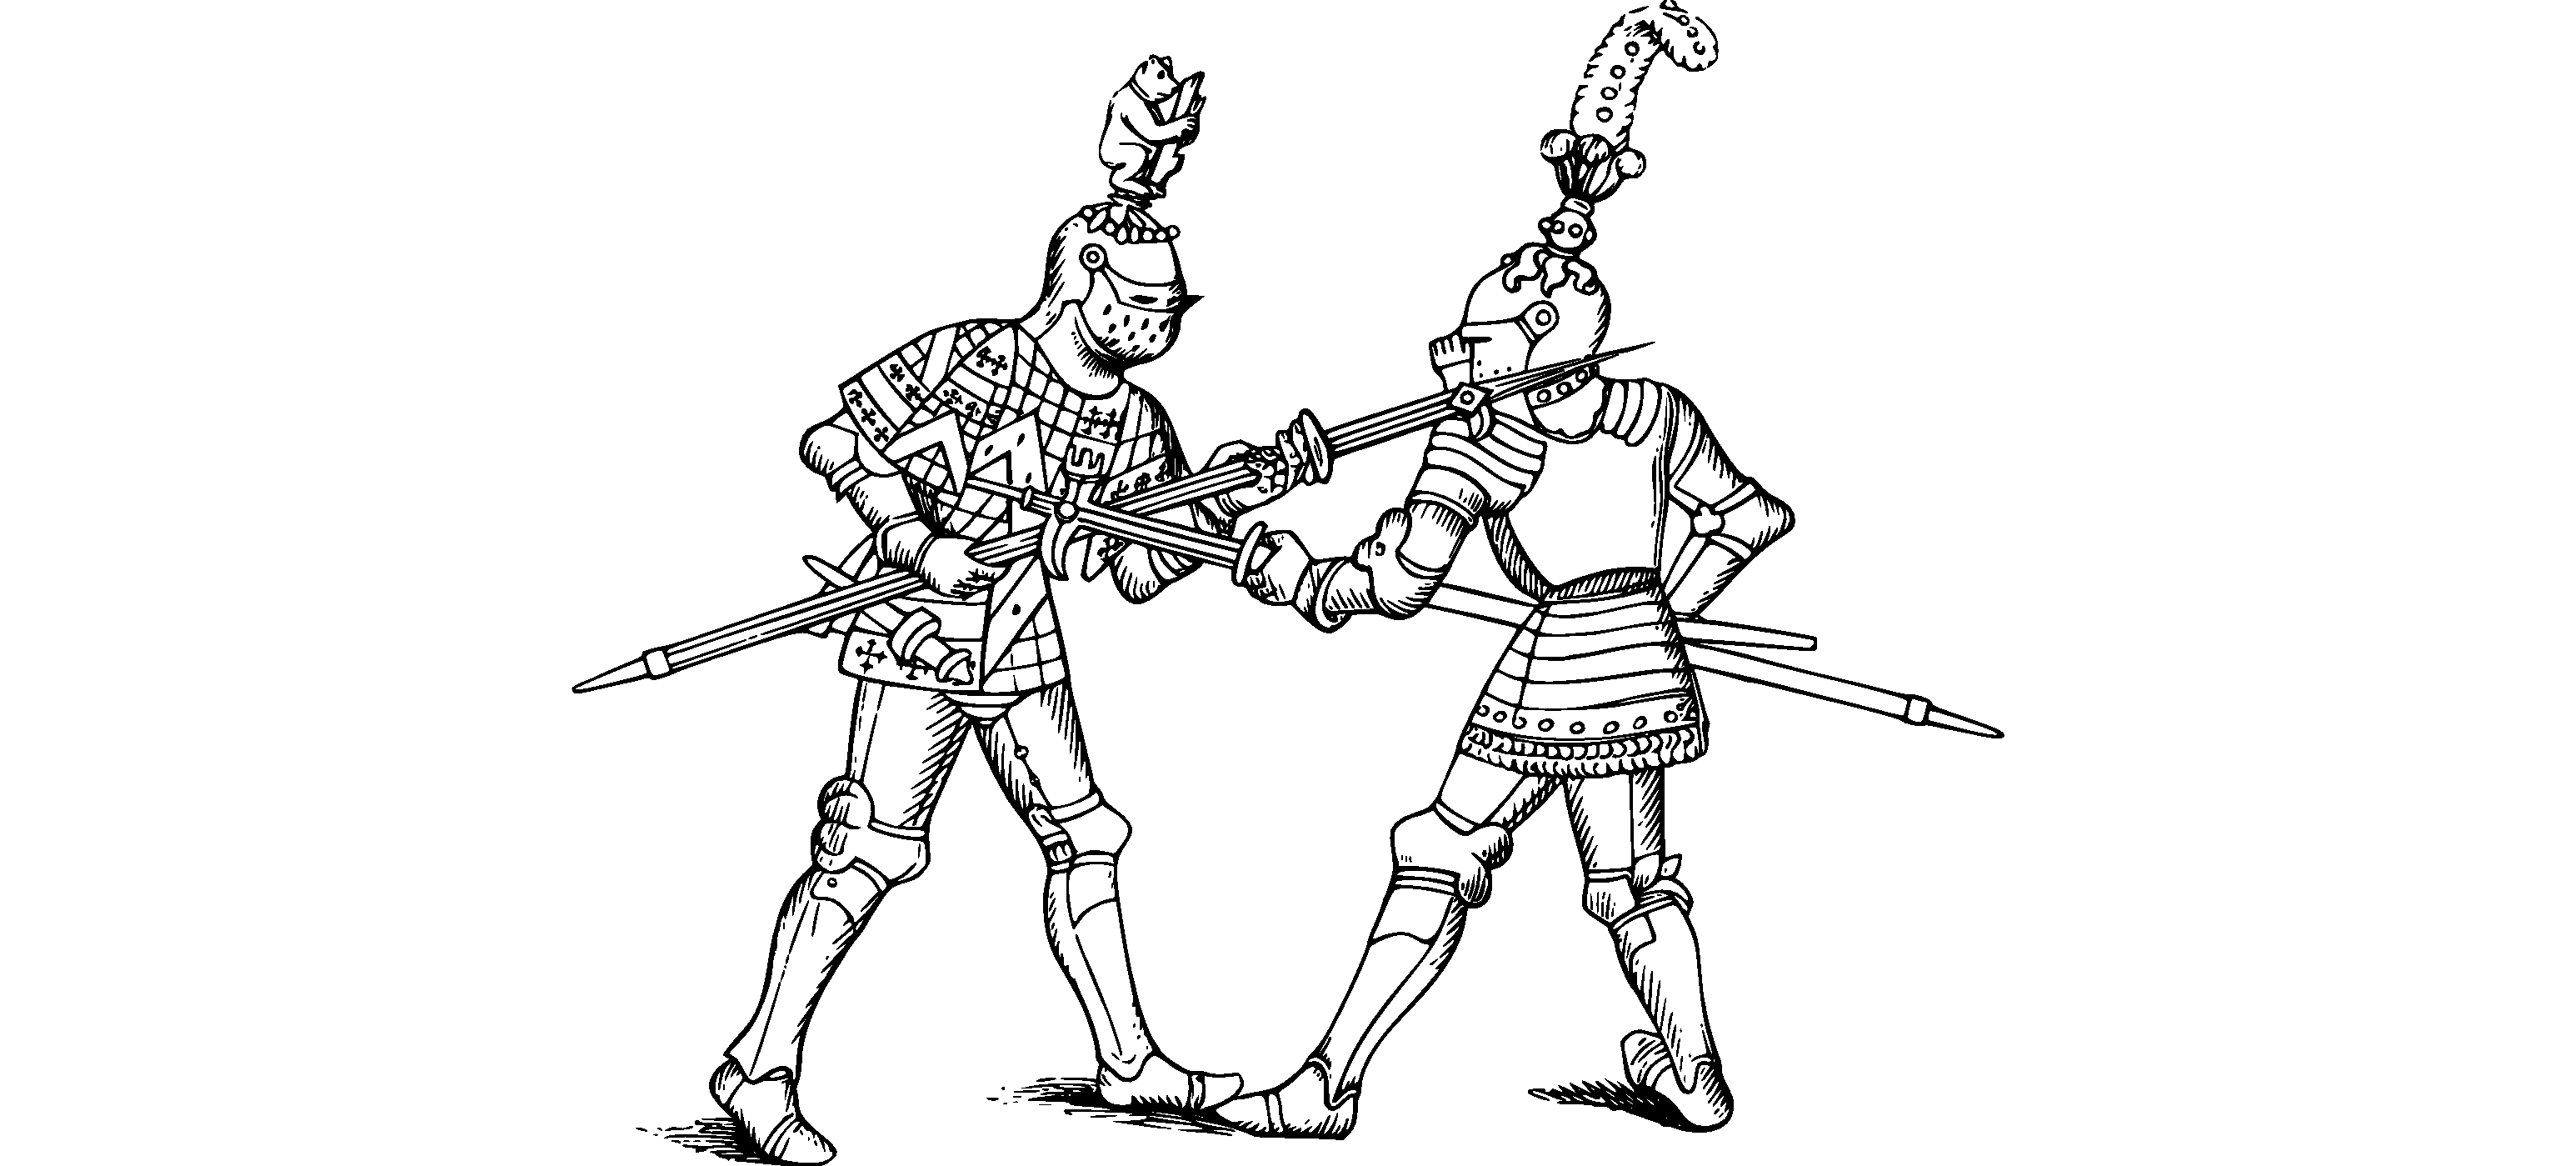
\includegraphics[width=\textwidth]{./images/presentation02.pdf}
    % \caption{Inline Example Image}
\end{figure}

Chapter 3: Survival Mechanics covers the mechanics of survival in Eidos, including food and water requirements, shelter, scavenging, travel, and exploration. Chapter 4: Character Injuries and Health provides a comprehensive guide to character injuries and health, including damage and wound mechanics, healing and recovery, status effects, and advanced injuries and trauma.

Chapter 5: Game Master Tools provides a guide to running Eidos games, including world-building, NPC generation, encounters, group dynamics, movement and travel, encounter generation, and campaign management. Chapter 6: Optional Rules and Variants covers alternative systems for combat, magic, and skills, as well as advanced mechanics for character development and progression and rules for playing in different settings and genres.

In conclusion, Eidos is an open source tabletop RPG system that offers a unique and engaging narrative experience, with mechanics that are designed to create immersive and exciting combat scenes. With its deep character creation process, engaging combat mechanics, and comprehensive survival mechanics, Eidos is a game that offers endless possibilities for players to explore and experience.

% ###################################################################################################
% Chapter 1 - Personality
% ###################################################################################################

\chapter{Personality}

% Chapter-wide image
\begin{center}
    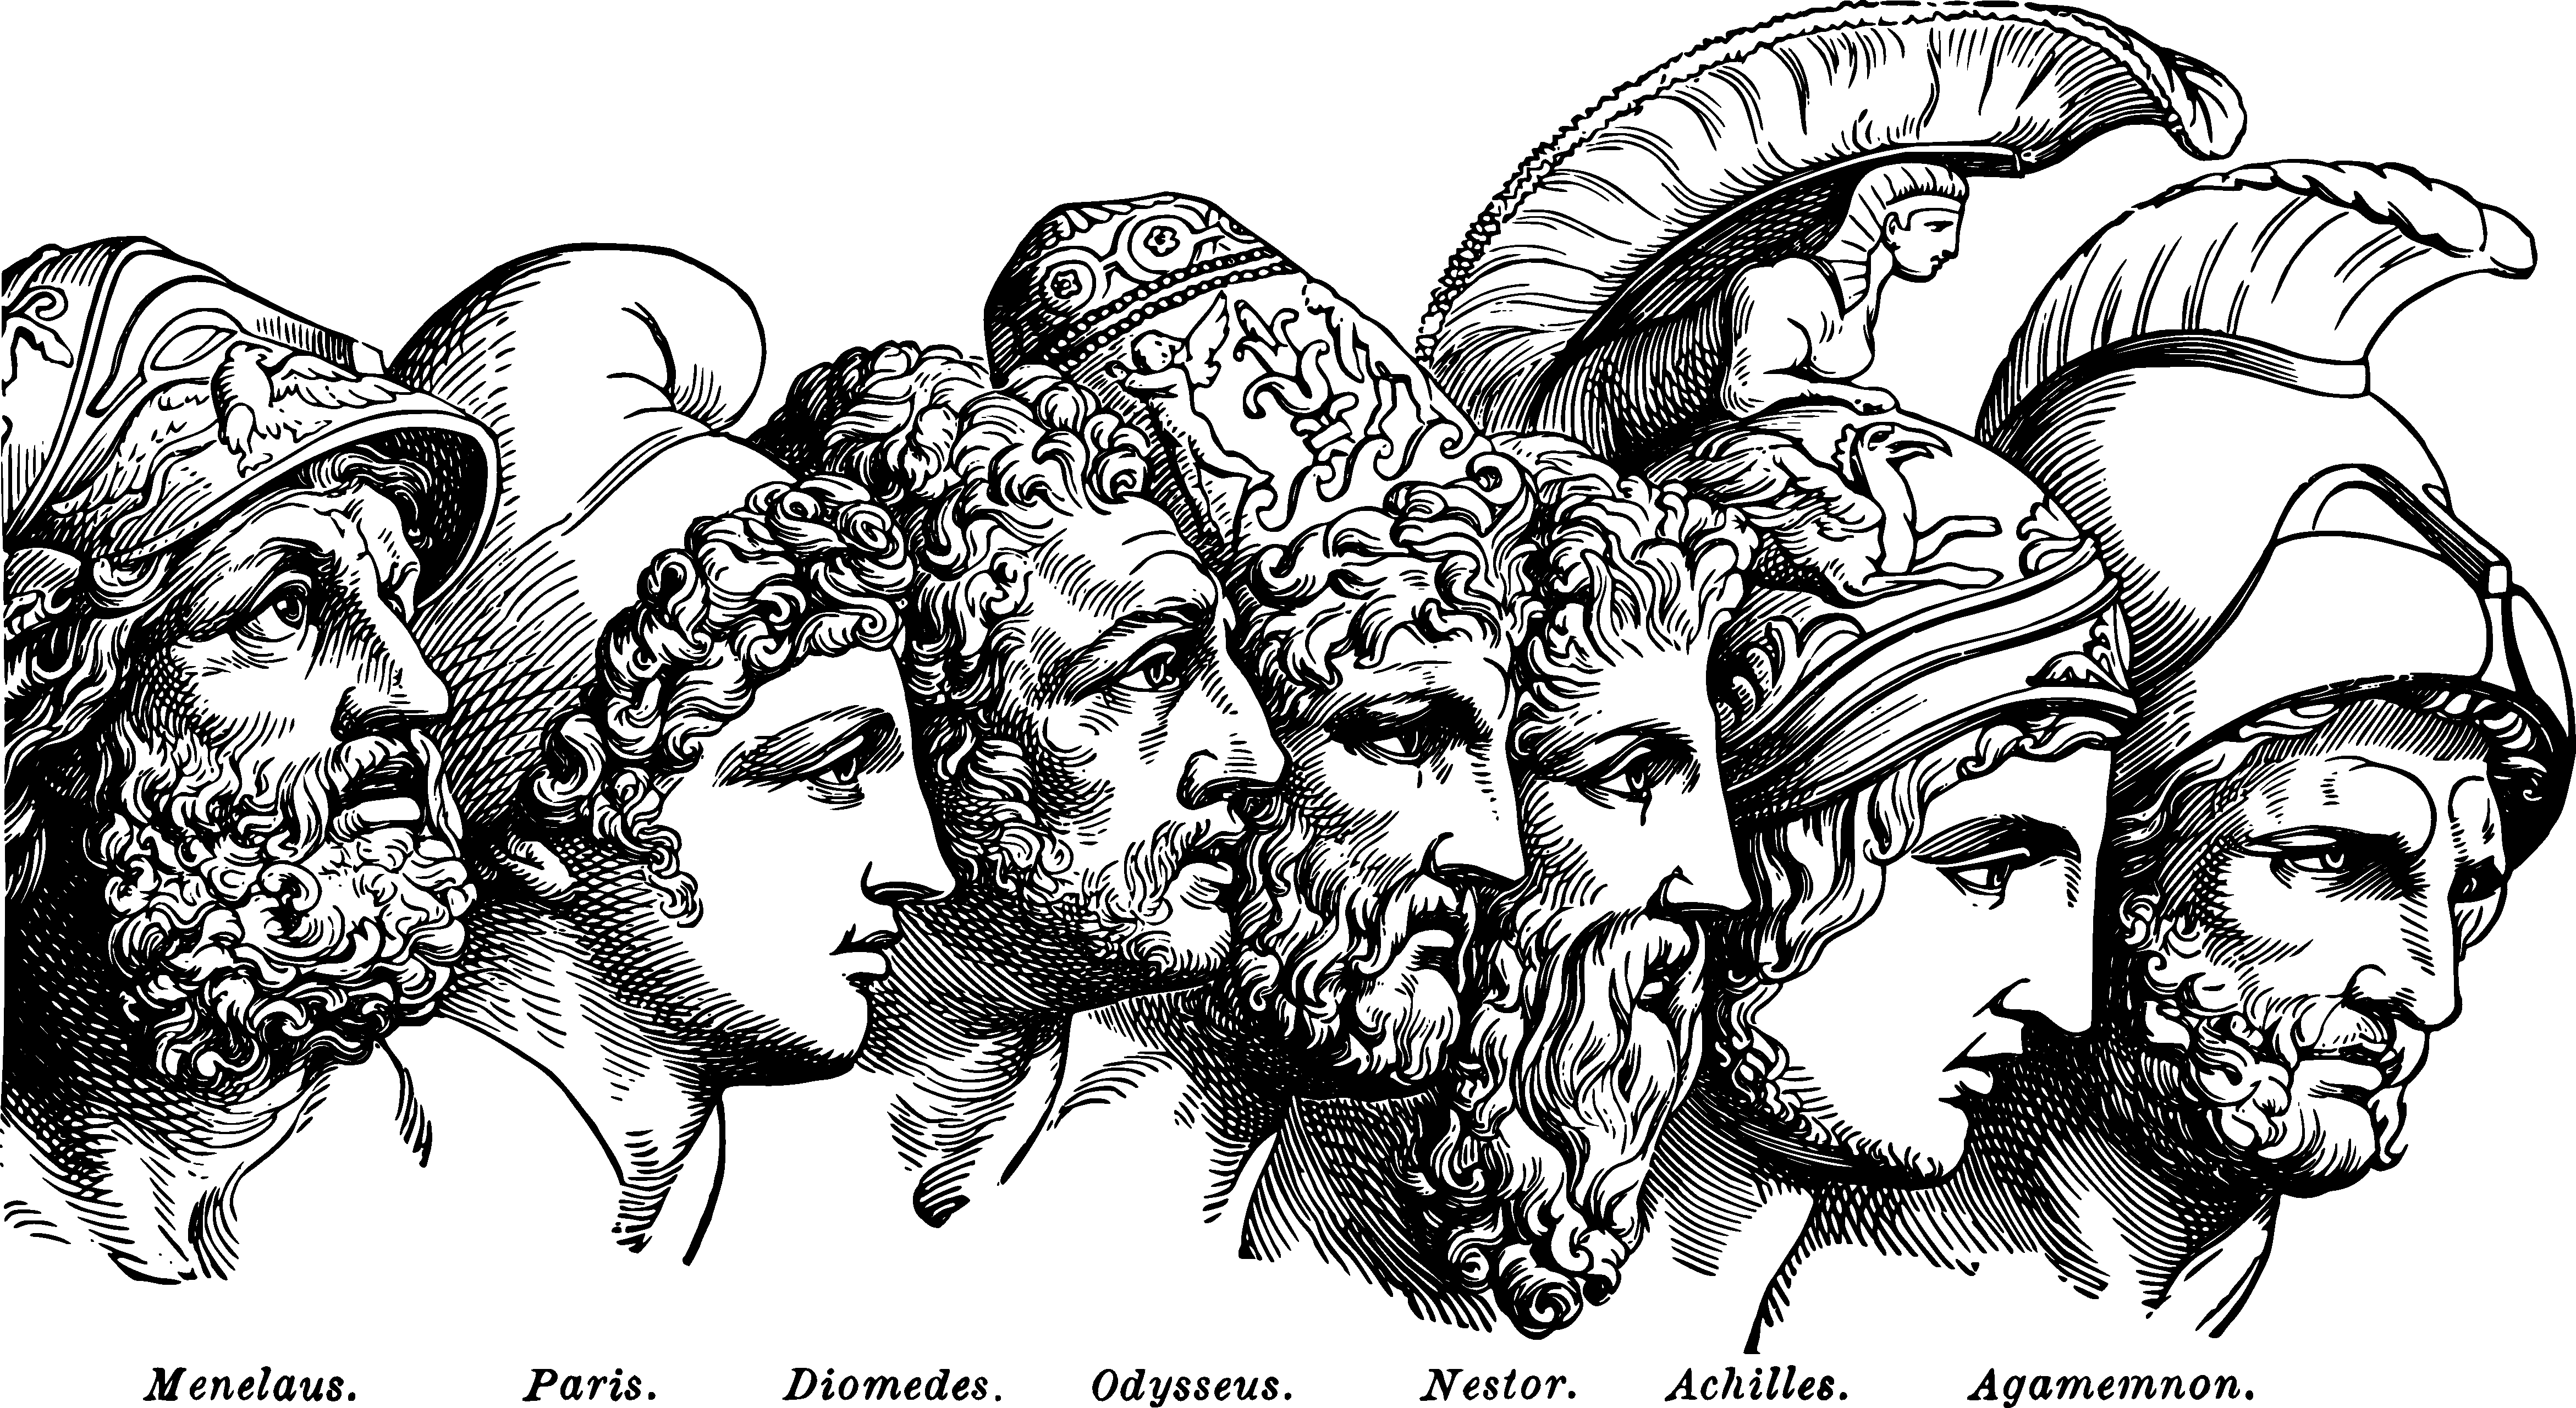
\includegraphics[width=\textwidth]{./images/personality01.pdf}
\end{center}

Most of this part will be based on [Ash’s Guide to RPG Personality \& Background](https://www.ashami.com/rpg/). Of course, some modifications will be needed to fit his tables into the system...

\subsection{\textbf{Primary Motivators}}

The first step in crafting a character's personality is selecting their primary and secondary motivators. These motivations serve as the driving force behind a character's actions and decisions, shaping the narrative of their journey. The primary motivator is particularly important, as it acts as the primary catalyst for a character's backstory and personality. It is the underlying theme of a character's motivations, guiding their behavior and propelling them forward.

When choosing these motivations, it's important to consider what your character wants most in the world. Is it wealth, power, love, revenge, or something else? By focusing on these motivations, players can ensure that their character's actions feel authentic and grounded in their personal desires. Whether facing challenges in combat or navigating complex social situations, characters driven by strong motivators will always have a clear direction and purpose.

\begin{description}
    \item[1. Achievement] To overcome obstacles and succeed; to become the best.
    \item[2. Acquisition] To obtain possessions/wealth.
    \item[3. Adoration] To be cherished, admired, and wanted by others.
    \item[4. Balance/Peace] To bring all things into harmony and equilibrium.
    \item[5. Beneficence] To protect the helpless, heal the sick, feed the hungry, etc.
    \item[6. Chaos] To disrupt, to cause confusion and discord.
    \item[7. Competition] To seek out or create rule-based win/lose scenarios; to defeat others in contests.
    \item[8. Conflict] To seek out or create rivalry, fighting, or animosity.
    \item[9. Conquest] To conquer other peoples, to bring them into one’s own culture/rule.
    \item[10. Corruption] To despoil, ruin, humiliate, or make depraved.
    \item[11. Creation] To build or make new, such as art, culture, invention, design, etc.
    \item[12. Destruction] To annihilate, exterminate, and unmake.
    \item[13. Discovery/Adventure] To explore, uncover mysteries, and pioneer.
    \item[14. Domesticity] To get married, have children, and live a family life.
    \item[15. Education] To provide information, teach, enlighten, or train.
    \item[16. Entertainment] To entertain, amuse, and delight others.
    \item[17. Enslavement] To force others into servitude.
    \item[18. Hedonism] To enjoy all things sensuous.
    \item[19. Heroism] To find valor and honor through battle or self-sacrifice.
    \item[20. Liberation] To free the self and/or others from perceived captivity or enslavement.
    \item[21. Love] To experience/share affection and emotional commitment, romantic or platonic.
    \item[22. Nobility/Honor] To exalt ideals such as generosity, honesty, bravery, and courtliness.
    \item[23. Order] To arrange, organize, and reduce chaos.
    \item[24. Play] To have fun, to enjoy life.
    \item[25. Power] To control and lead others.
    \item[26. Proselytization] To spread a belief system; indoctrinate others.
    \item[27. Purity] To achieve a state of moral or spiritual perfection, of self and/or others.
    \item[28. Rebellion] To fight against power structures; to undermine authority.
    \item[29. Recognition] To gain approval, social status, or fame.
    \item[30. Service] To follow a person, government, order, religion, etc.
    \item[31. Torment] To inflict pain and suffering, on others and/or the self.
    \item[32. Understanding] To seek knowledge or wisdom (spiritual, scientific, magical, etc).
    \item[33. Vice] To enable or engage in self-destructive behavior.
\end{description}

\begin{figure}[h]
    \centering
    \includegraphics[width=\textwidth]{./images/personality02.pdf}
    % \caption{Inline Example Image}
\end{figure}

\subsection{\textbf{Dispositions}}

Disposition is an important aspect of character creation that provides depth and dimension to your character's personality. It allows you to understand how your character is likely to react emotionally to different situations, as well as how they appear to others. This trait helps you create a believable and relatable character, giving them an emotional landscape that makes sense within the context of the story.

When determining your character's emotional disposition, it is important to keep in mind that it is not necessarily limiting. It simply provides a baseline for how your character is likely to feel at any given moment. A character with a predominantly cheerful disposition may still experience moments of sadness, anger, or anxiety, but they will be more likely to return to their cheerful state after those moments have passed.

It is also important to note that emotional disposition should not be equated with alignment. A character's disposition can exist independently of their moral or ethical alignment, and it is possible for a character to be joyfully evil or angrily good. Understanding your character's disposition will help you make decisions about their emotional reactions, but it is just one aspect of the complex and multifaceted personality that you are creating.

\begin{enumerate}
    \item Joyful
    \item Anxious
    \item Melancholy
    \item Curious
    \item Calm
    \item Angry
    \item Contemptuous
    \item Excited
    \item Apathetic
    \item Ashamed
\end{enumerate}

\subsection{\textbf{Moodiness}}

Moodiness is an important aspect of a character's personality and can greatly impact their behavior in different situations. A character who is labile, or quick to experience intense emotions, is likely to react strongly to the events happening around them. This can make them appear impulsive and prone to outbursts, but it can also add a level of excitement and unpredictability to their actions. On the other hand, a phlegmatic character, who is psychologically consistent and moderate, is likely to maintain their composure in even the most trying of situations. This calm demeanor can give them a sense of stability and reliability, but it can also make them appear uninterested or indifferent to the world around them.

It is important to note that both moodiness traits have their own strengths and weaknesses, and they can greatly impact a character's relationships with other characters. For example, a labile character may be prone to jealousy or resentment, while a phlegmatic character may struggle with expressing their emotions effectively. Choosing the right moodiness trait for your character can help you build a more complete and well-rounded personality.

Ultimately, the key to making a character's moodiness work for them is understanding the underlying motivations and dispositions that drive their behavior. Whether your character is quick to experience intense emotions or stays calm and collected in the face of adversity, the key is to make sure that their moodiness feels true to who they are as a character. By incorporating moodiness into your character's personality, you can add depth and richness to your role-playing experience and help bring your character to life on the tabletop.

\begin{enumerate}
    \item Labile
    \item Even-tempered
    \item Phlegmatic
\end{enumerate}

\begin{figure}[h]
    \centering
    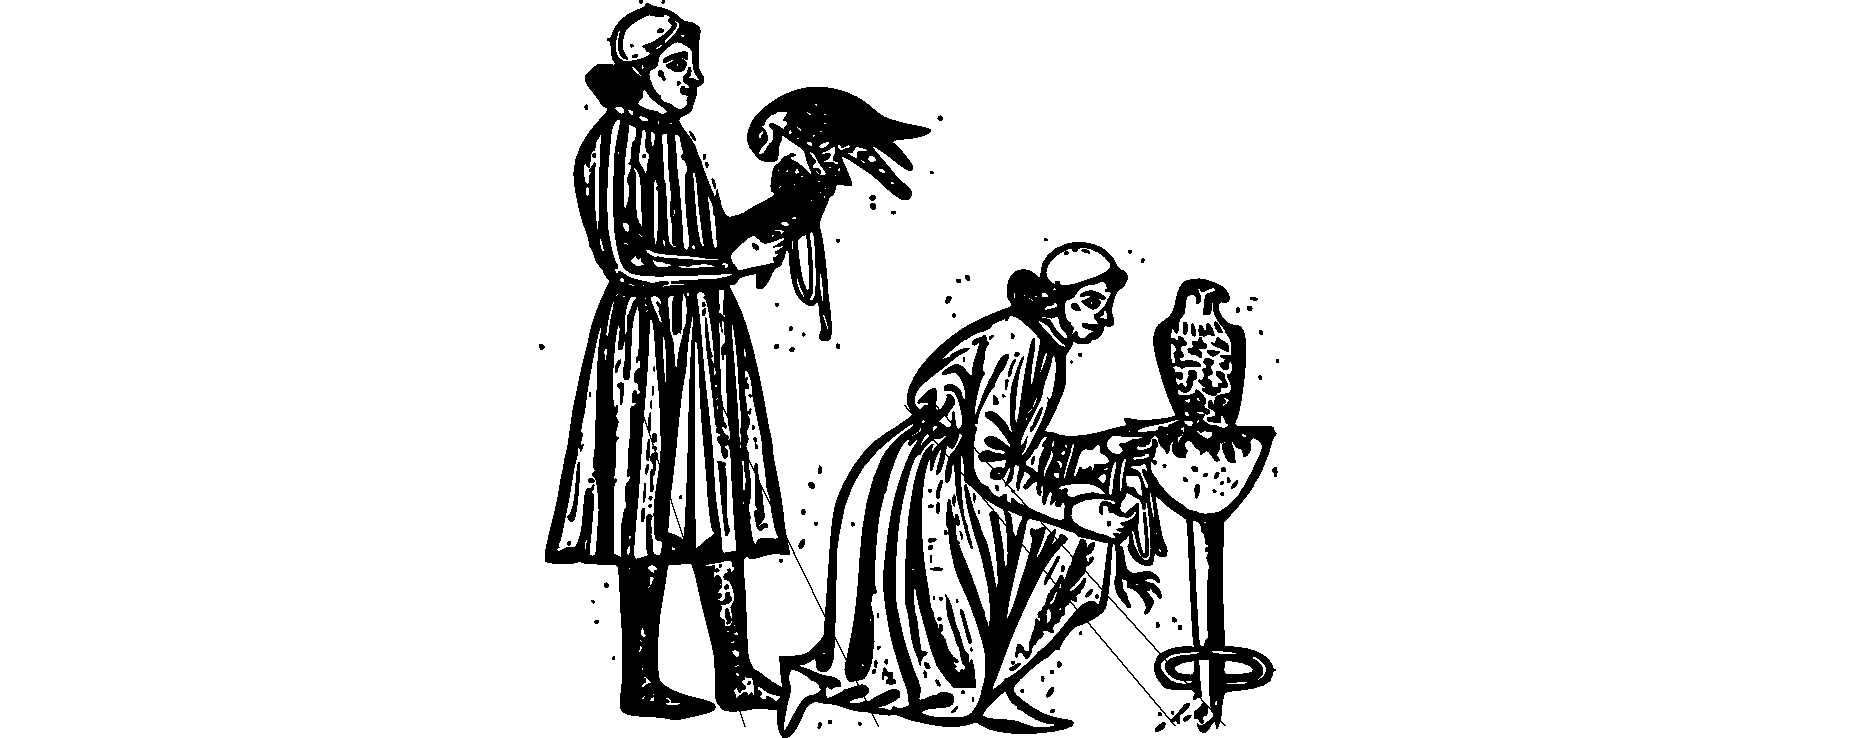
\includegraphics[width=\textwidth]{./images/personality03.pdf}
    % \caption{Inline Example Image}
\end{figure}

\subsection{\textbf{Outlook}}

The concept of outlook is an important aspect of character creation as it defines the basic worldview of a character and helps determine their overall view of the world around them. This trait can greatly influence the choices that a character makes and the way they interact with others. A character with a positive outlook is likely to see the good in people and situations, while a character with a negative outlook is likely to be more skeptical and pessimistic. Understanding a character's outlook is key to understanding their motivations and how they may react in different situations. It is important to note that a character's outlook does not dictate their alignment, as a character can have a positive outlook but still make morally questionable decisions. This trait helps to add depth and complexity to a character, making them feel more real and unique.

\begin{description}
    \item[Optimistic] An optimistic outlook is characterized by idealism and confidence. Individuals with this outlook tend to be trusting and hopeful, often viewing situations with an upbeat attitude and a positive expectation for outcomes.
    \item[Pessimistic] A pessimistic outlook is often marked by cynicism and a bleak perspective. Those with this outlook may be distrustful and foreboding, expecting negative outcomes and sometimes feeling resigned to unfavorable situations.
    \item[Realistic] A realistic outlook is grounded in practicality and balance. Realistic individuals approach situations pragmatically, focusing on what is achievable and maintaining a level-headed perspective.
\end{description}

\subsection{\textbf{Integrity}}

Integrity refers to the values that guide a character's behavior in work and social interactions. When creating a character, players can choose between two options that embody different qualities and tendencies. The first option is "Conscientious", which represents being industrious, honest, responsible, meticulous, and pragmatic. On the other hand, the second option is "Unscrupulous", which embodies being lazy, deceitful, unreliable, manipulative, slipshod, and impractical. These two options serve as a starting point for players to develop their character's personality and decision-making. The choice of integrity will play a crucial role in determining a character's motivations and actions, influencing the character's interactions with others and the events of the story.

\begin{description}
    \item[Conscientious] The individual is industrious, honest, responsible, meticulous, and pragmatic.
    \item[Unscrupulous] The individual is lazy, deceitful, unreliable, manipulative, slipshod, and impractical.
\end{description}

\begin{figure}[h]
    \centering
    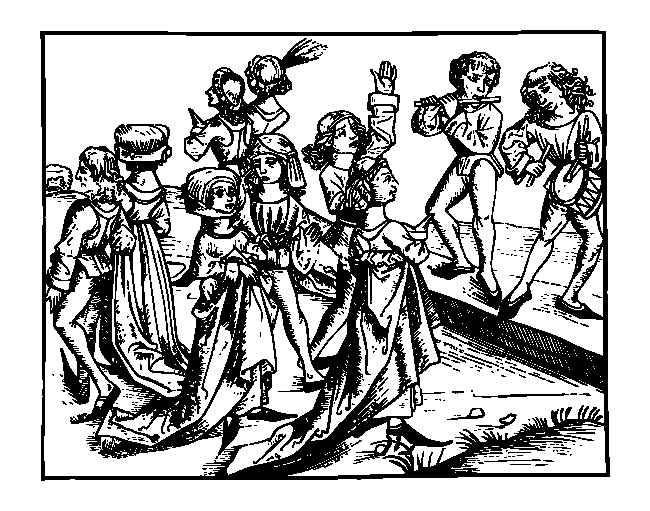
\includegraphics[width=\textwidth]{./images/personality04.pdf}
    % \caption{Inline Example Image}
\end{figure}

\subsection{\textbf{Impulsiveness}}

The next aspect of character creation to consider is impulsiveness. This trait refers to a character's ability to regulate their thoughts and actions. Players must choose between two options: controlled or spontaneous. A controlled character is deliberate, focused, steady, and thoughtful. They carefully consider their decisions and think before they act. On the other hand, a spontaneous character is capricious, flighty, hyperactive, and rash. They are quick to act without thinking through the consequences of their actions. It's important to consider impulsiveness as it can greatly impact the way a character approaches situations and reacts to stimuli. A controlled character may be more reliable and level-headed, while a spontaneous character may be more unpredictable and exciting. Ultimately, the choice of impulsiveness helps to round out a character's personality and inform their behavior.

\begin{description}
    \item[Controlled] The individual is deliberate, focused, steady, and thoughtful in their actions.
    \item[Spontaneous] The individual tends to be capricious, flighty, hyperactive, and rash in their behavior.
\end{description}

\subsection{\textbf{Boldness}}

When it comes to creating a character's personality, it is important to consider their boldness, or willingness to face danger and enter into battle. This trait can greatly impact how a character approaches conflict and adversity, and can inform their actions and decisions in high-pressure situations. There are two main options for this characteristic: intrepid and cautious.

Intrepid characters are daring, reckless, and valorous. They have a confident demeanor and are not easily intimidated by danger. They are known for their bravery and audacity in the face of adversity, and are often seen as leaders in combat situations. On the other hand, cautious characters are timid, paranoid, and vigilant. They are nervous and tentative in the face of danger, preferring to assess the situation before making a move. They are not as quick to jump into action, but their carefulness can often lead to a more strategic approach to conflict.

\begin{description}
    \item[Intrepid] The individual is daring, reckless, valorous, dauntless, audacious, and confident.
    \item[Cautious] The individual is timid, paranoid, vigilant, nervous, and tentative in their actions.
\end{description}

\begin{figure}[h]
    \centering
    \includegraphics[width=\textwidth]{./images/personality05.pdf}
    % \caption{Inline Example Image}
\end{figure}

\subsection{\textbf{Agreeableness}}

The sub-topic of "Agreeableness" deals with a character's overall attitude towards others and their ability to handle interpersonal conflicts and new situations. This trait is particularly important in shaping a character's behavior in social interactions and their ability to navigate challenging circumstances. A character who is described as "Agreeable" is warm, empathetic, and open-minded, possessing qualities such as tolerance, forgiveness, and adaptability. On the other hand, a character who is described as "Disagreeable" is cold and rigid, possessing traits such as tension, intractability, and narrow-mindedness. Understanding a character's level of agreeableness can give insight into how they are likely to respond in social and interpersonal situations.

\begin{description}
    \item[Agreeable] The individual is warm, empathetic, tolerant, forgiving, open-minded, adaptable, and altruistic.
    \item[Disagreeable] The individual is cold, rigid, tense, intractable, narrow-minded, cantankerous, and stingy.
\end{description}

\subsection{\textbf{Interactivity}}

The next sub-topic in character creation is Interactivity, which deals with the way your character interacts with others. This aspect of personality is crucial in shaping the character's social relationships and determining how they engage with the world around them. The table of choices in Interactivity includes two options: Engaging and Reserved. An Engaging character is often talkative, candid, and touchy, while a Reserved character is usually shy, preferring to keep to themselves and be more reserved in their interactions. Understanding this aspect of your character will greatly enhance the depth of your role-playing experience and allow you to build compelling, engaging stories.

\begin{description}
    \item[Engaging] The individual is talkative, candid, entertaining, and touchy.
    \item[Reserved] The individual is shy, a loner, taciturn, evasive, and cryptic.
\end{description}

\subsection{\textbf{Conformity}}

Conformity is an important aspect of a character's personality, determining their relationship with cultural norms and societal expectations. A character who is conventional is likely to follow orthodox beliefs and practices, be formal in their demeanor, and adhere to mainstream customs. On the other hand, a character who is heterodox may be rebellious in nature, have a creative and artistic streak, and may be known for their freethinking and exotic choices. Understanding a character's conformity can give insight into how they view and interact with the world around them.

\begin{description}
    \item[Conventional] The individual is orthodox, formal, down-to-earth, mainstream, and traditional.
    \item[Heterodox] The individual is rebellious, arty, shocking, freethinking, and exotic.
\end{description}

\subsection{\textbf{Quirks, Habits, and Oddities}}

To help bring your character to life and add depth to gameplay, consider incorporating small quirks, habits, and oddities into their personality. These unique behavioral characteristics can range from relatively harmless habits, such as humming or lip biting, to more engaging and potentially entertaining quirks such as exhibitionism or sleepwalking. By adding these small but meaningful details to your character, you can bring them to life in a way that sets them apart from the rest of the party.

These quirks, habits, and oddities can offer a multitude of role-playing opportunities. They can help flesh out a character's backstory, provide unique challenges or benefits during gameplay, and even influence the way they interact with other characters. For example, a character who is a compulsive liar may struggle with building trust with others, while a character who is an animal hater may have trouble working with characters who have animal companions. Whether you choose to focus on the more harmless or more engaging quirks, incorporating these small behaviors into your character can greatly enhance your role-playing experience.

\begin{multicols}{2} % Start two-column layout
    \begin{enumerate}
        \item Humming
        \item Dancing
        \item Sleepwalking
        \item Facial tics
        \item Exhibitionism
        \item Fingernail biting
        \item Eavesdropping
        \item Daydreaming
        \item Talking in sleep
        \item Stuttering
        \item Compulsive lying
        \item Whistling
        \item Name dropping
        \item Self-inflict pain/injury
        \item Mumbling
        \item Constant grooming
        \item Foot tapping
        \item Lip biting/licking
        \item Coin flipping
        \item Chewing (e.g. sticks, small bones)
        \item Knuckle cracking
        \item Collects odd things
        \item Singing
        \item Snacking (nuts, seeds, etc.)
        \item Reciting poetry
        \item Constant eating
        \item Pacing
        \item Blade sharpening
        \item Counting
        \item Hair pulling
        \item Snoring
        \item Walking backwards
        \item Teeth sucking
        \item Excessively touching others
        \item Substance use (non-addicted)
        \item Animal hater
        \item Insomnia
        \item Beard/hair stroking
        \item Nose picking
        \item Needless apologizing
        \item Exaggeration
        \item Superstitious (omens, luck, etc.)
        \item Belching
        \item Sleeping in odd places
        \item Repeating others
        \item Smelling things
        \item Teeth picking
        \item Stealing
        \item Tree climbing
        \item Excessive sweating
        \item Nervous laughter
        \item Touching/tugging earlobes
        \item Twirling hair/beard
        \item Playing with objects
        \item Biting tongue/lips
        \item Nail tapping
        \item Constant yawning
        \item Blinking excessively
        \item Bouncing legs
        \item Skipping/hopping
        \item Clearing throat repeatedly
        \item Covering mouth while speaking
        \item Fidgeting with hands
        \item Whispering to self
        \item Nervous nail biting
        \item Licking/smacking lips
        \item Staring blankly
        \item Chewing gum
        \item Sighing heavily
        \item Breathing heavily
        \item Scratching self
        \item Clicking pen/tapping fingers
        \item Swallowing hard
        \item Clearing throat loudly
        \item Tapping feet
        \item Fidgeting with clothing
        \item Avoiding eye contact
        \item Glancing around nervously
        \item Talking too fast/slow
        \item Stuttering words
        \item Twitching facial muscles
        \item Rubbing hands together
        \item Biting cheek/tongue
        \item Staring off into space
        \item Nodding/shaking head excessively
        \item Interrupting others
        \item Leaning in too close
        \item Speaking loudly
        \item Repeating words/phrases
        \item Rocking back and forth
    \end{enumerate}
    \end{multicols}
    
\begin{figure}[h]
    \centering
    \includegraphics[width=\textwidth]{./images/personality06.pdf}
    % \caption{Inline Example Image}
\end{figure}

\subsection{\textbf{Sense of Humor}}

Sense of Humor is an important aspect of a character's personality and can be used to show their humor preferences and how they might react in different situations. It ranges from crude humor to dry wit and includes various styles such as slapstick, jokey, cynical, prankster, mean-spirited, gleeful, and surreal. By selecting one of these options, you can help to define your character's sense of humor and how they might react in different situations. Having a strong sense of humor can also be a way for your character to diffuse tense situations, and can be used to show their lighter side. Ultimately, your character's sense of humor is a tool that you can use to further develop their personality and bring them to life in your storytelling.

\begin{enumerate}
    \item Crude
    \item Dry
    \item Slapstick
    \item Jokey
    \item Cynical
    \item Prankster
    \item Mean-spirited
    \item Gleeful
    \item Surreal
\end{enumerate}

\subsection{\textbf{Mental Disorders}}

In this RPG system, we aim to provide an accurate representation of human mental and emotional disorders. While we understand that not all players may want their character to struggle with such issues, it does present an opportunity for unique and interesting role-play. For this reason, we suggest that players consider assigning these disorders to non-player characters, adding depth and complexity to the game world. It's important to note that the list provided is not exhaustive and only offers brief descriptions. Nevertheless, these disorders can also serve as inspiration for creating realistic and terrifying curses or divine punishments.

\begin{enumerate}
    \item \textbf{Addiction:} Chronic, compulsive drug/activity indulgence, despite harmful consequences. Can decide if it is mild, moderate, or severe.
    \item \textbf{Amnesia:} Severe memory loss; can be loss before a certain point (retrograde) or after (anterograde).
    \item \textbf{Bipolar Disorder:} Erratic swings from periods of mania to major depression.
    \item \textbf{PTSD:} Anxiety disorder developed after exposure to a terrifying event or ordeal resulting in potential re-experiencing of the ordeal, nightmares, hypervigilance, trouble sleeping, being easily startled, and avoidance of anything that is a reminder of the event.
    \item \textbf{Major Depression:} Impaired physical functions (e.g., sleep, appetite); loss of interest and pleasure; low energy \& motivation; possibly accompanied by severe pessimism, hopelessness, guilt, and suicidal thoughts/intent.
    \item \textbf{Fugue:} Abrupt travel away from home, an inability to remember important aspects of one’s life, and the partial or complete adoption of a new identity.
    \item \textbf{Hypochondria:} Preoccupation with fears of having a serious disease or physical problem based on little or no real evidence.
    \item \textbf{Schizophrenia:} Delusions (unreal beliefs, e.g., savior complex or assigning unusual significance or meaning to normal events); hallucinations (unreal sensations, usually auditory, i.e., “voices”); disorganized speech; grossly disorganized or catatonic behavior; paranoia.
    \item \textbf{OCD:} Obsessive-Compulsive Disorder described the existence of both regular compulsions (overwhelming need to engage in a ritualized behavior) and obsessions (persistent, often irrational, and seemingly uncontrollable thoughts).
    \item \textbf{Phobia:} Extreme anxiety and fear associated with an object or situation. Can include anything, for instance: specific monsters/animals, fire/water, heights, magic, open/enclosed spaces, heights, or darkness.
    \item \textbf{Agoraphobia:} Fear of being in a situation where escape is difficult or where help might not be available in the event of a panic attack or other medical emergency.
    \item \textbf{Social Anxiety Disorder:} Extreme fear of embarrassment or criticism in social situations.
    \item \textbf{Body Dysmorphic Disorder:} Preoccupation with an imagined or minor defect in one’s appearance.
    \item \textbf{Generalized Anxiety Disorder:} Chronic, excessive worry about multiple life events and activities.
    \item \textbf{Obsessive Love Disorder:} Intrusive thoughts about an individual and an overwhelming need to be with them.
    \item \textbf{Delusional Disorder:} A condition in which an individual experiences non-bizarre delusions, meaning the delusions are not implausible and could happen in reality.
    \item \textbf{Adjustment Disorder:} Disturbance caused by a specific stressful life event, such as a loss, change in lifestyle, or change in health status.
    \item \textbf{Narcissistic Personality Disorder:} Excessive self-love, entitlement, and a lack of empathy for others.
    \item \textbf{Borderline Personality Disorder:} A pattern of instability in relationships, moods, self-image, and behavior.
    \item \textbf{Antisocial Personality Disorder:} A disregard for laws and the rights of others.
    \item \textbf{Anxiety Disorder:} A general term for excessive fear or worry about everyday events and activities.
    \item \textbf{Dissociative Identity Disorder:} A pattern of unstable emotions, relationships, and sense of self.
    \item \textbf{Histrionic Personality Disorder:} A condition in which a person's sense of identity is fragmented and they experience two or more distinct and alternating personalities.
    \item \textbf{Obsessive-Compulsive Personality Disorder:} A pattern of excessive emotionality and attention-seeking behavior.
    \item \textbf{Paranoia:} A pattern of preoccupation with orderliness, perfectionism, and control.
    \item \textbf{Psychotic Disorder:} A pattern of grandiosity, need for admiration, and lack of empathy.
    \item \textbf{Eating Disorder:} An unreasonable distrust or suspicion of others, often accompanied by delusions.
    \item \textbf{Trichotillomania:} A group of mental illnesses characterized by distorted thinking, perceptions, emotions, and behaviors.
\end{enumerate}

\subsection{\textbf{Topics of Conversation}}

One helpful way to bring depth to your character is to determine what they like to talk about in casual social situations. People are naturally inclined to talk about things they are skilled in or have a personal interest in, and this is an easy way to help flesh out your character. By examining your character's skills, hobbies, training, and background, you can start to determine what topics they might be passionate about. This information can be used to create a more complete picture of who your character is and how they interact with others in social situations. By giving your character a few key topics they like to discuss, you can help bring them to life and make them more memorable to other players.

\subsection{\textbf{Conclusion}}

In conclusion, the character's personality is a crucial aspect in role-playing games and helps to bring the character to life. This chapter has covered a range of fields that allow players to flesh out their characters, including alignment, morality, values, beliefs, religion and spirituality, and quirks. These fields provide a comprehensive and nuanced view of the character's personality, allowing players to bring depth and dimension to their characters. By taking the time to fill out these fields, players can create truly unique and engaging characters that will bring their stories to life. Whether playing a heroic warrior or a cunning rogue, these fields help players to truly embody their characters and bring the world of the game to life.

% ###################################################################################################
% Chapter 2 - Spirituality and Religion
% ###################################################################################################

\chapter{Spirituality and Religion}

% Chapter-wide image
\begin{center}
    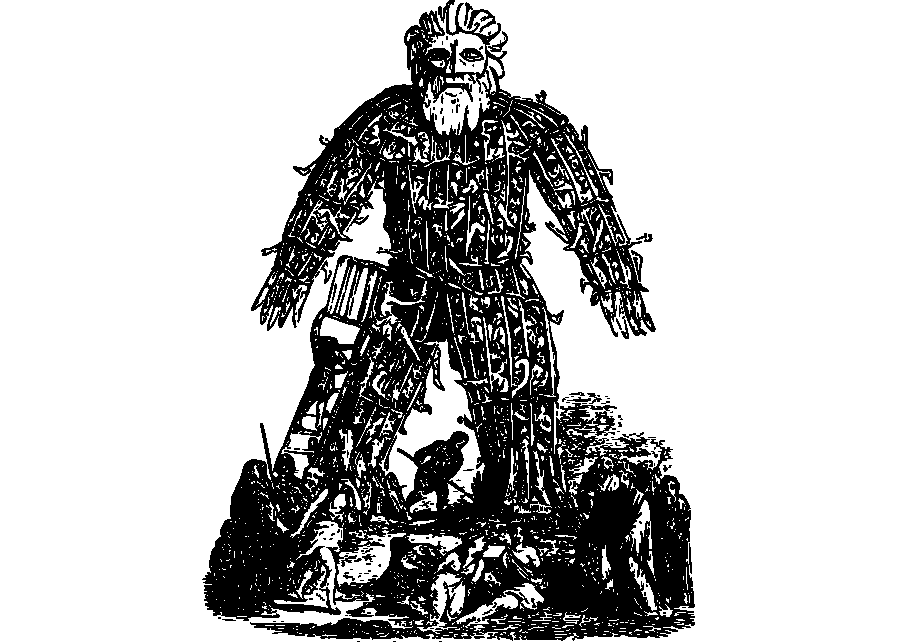
\includegraphics[width=\textwidth]{./images/religion01.pdf}
\end{center}

In the world of role-playing games, it's important to consider the spirituality and religious beliefs of a character. The Spirituality Sheet is an integral part of character creation and is designed to help players define their character's connection to the spiritual and religious aspects of the game world. This chapter will detail the mechanics behind the Spirituality Sheet, including the options available for defining the strength of a character's belief or association with a religious system, as well as any relevant traits and skills that may impact the character's spirituality and religious beliefs. Whether playing as a devout follower of a particular faith or a non-believer, the Spirituality Sheet will help players bring their character to life and create a more immersive role-playing experience.

\subsection{\textbf{Adherence}}

The "Adherence" field on the character sheet represents the strength of the character's belief or association with a particular religious or spiritual system. The options for this field range from non-believer to orthodox adherent, providing a spectrum of beliefs that a character can possess. The non-believer is someone who does not hold any belief in a higher power, whereas an agnostic is someone who is uncertain about the existence of a higher power. On the other hand, a casual adherent is someone who holds a loose connection to their religious or spiritual beliefs, and an orthodox adherent is someone who strictly follows the teachings and practices of their chosen system. This mechanic helps to further flesh out the character and their motivations, and provides a lens through which the character may view the world around them.

\begin{enumerate}
    \item Non-believer
    \item Agnostic
    \item Casual adherent
    \item Orthodox adherent
\end{enumerate}

\subsection{\textbf{Tolerance}}

This field reflects the character's willingness to accept differences of belief in others. In determining the level of tolerance, there are three options available for the player to choose from: Inclusive, Tolerant, or Intolerant. The level of tolerance selected will affect how the character interacts with people of different beliefs and religions in the game world.

\begin{enumerate}
    \item Inclusive
    \item Tolerant
    \item Intolerant
\end{enumerate}

\begin{figure}[h]
    \centering
    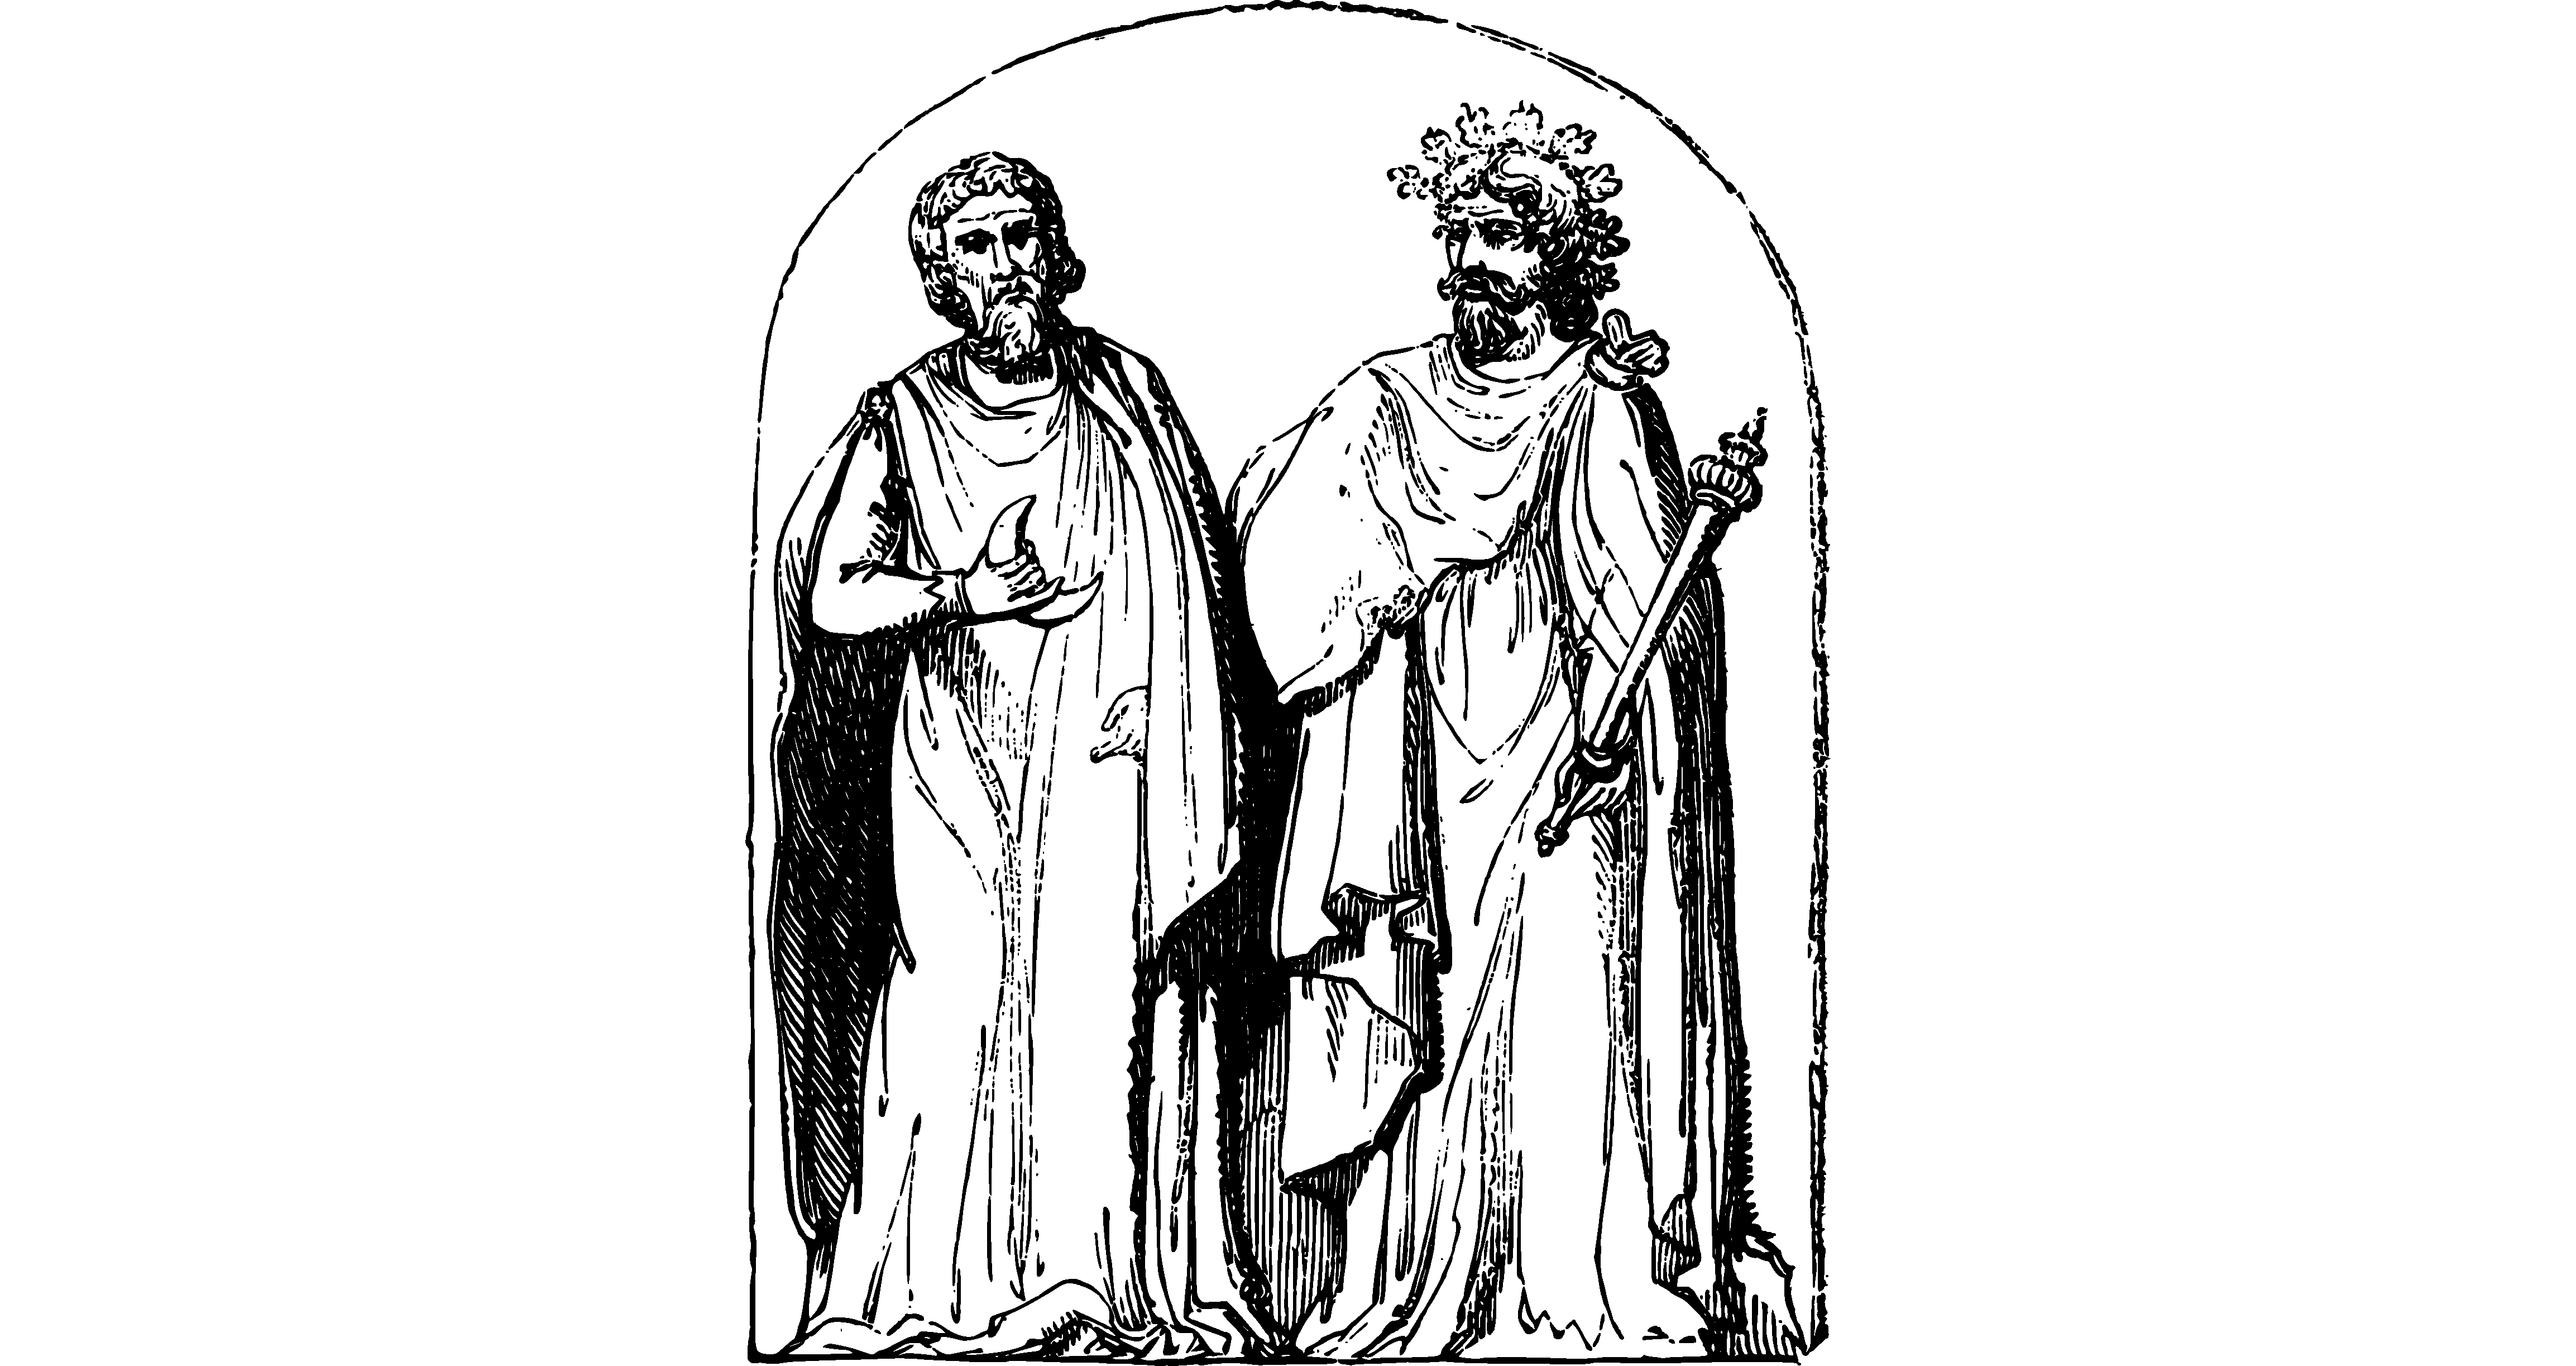
\includegraphics[width=\textwidth]{./images/religion03.pdf}
    % \caption{Inline Example Image}
\end{figure}

\subsection{\textbf{Religious Demeanor}}

The field "RELIGIOUS DEMEANOR" on the character sheet aims to capture how your character tends to act in regards to religious beliefs. To reflect this, the player will be presented with three different fields to fill out. The first field is "Expression of beliefs" and asks the player to decide on the frequency at which their character expresses their beliefs. The options range from "None", "Occasional", to "Constant". The next field is "Converting others", which asks the player to choose the level of effort the character puts into converting others to their beliefs. The choices here are "Never", "Casual", and "Aggressive". Finally, the "Attitude" field asks the player to choose the general approach the character takes towards religion and religious beliefs. The options for this field range from the irreverent "Irreverent" to the devout "Ecstatic". By filling out these fields, the player can gain a deeper understanding of their character's relationship to religion and spirituality.

\textbf{Expressions of Beliefs:} The individual may express their beliefs in different ways. They could be a \textbf{\textit{None}}, meaning they do not express their beliefs outwardly. They could be \textbf{\textit{Occasional}}, meaning they express their beliefs casually or sporadically. Or, they could be \textbf{\textit{Constant}}, meaning they frequently and openly express their beliefs.

\textbf{Approach to Converting Others:} When it comes to converting others, individuals may approach this in varying degrees. They might be \textbf{\textit{Never}} interested in converting others to their beliefs, meaning they have no desire to do so. They might be \textbf{\textit{Casual}}, where they casually discuss their beliefs with others without the intent to convert them. Or, they might be \textbf{\textit{Aggressive}}, meaning they actively try to convert others, sometimes with strong persuasion.

\textbf{Attitudes Toward Beliefs:} Individuals also differ in how they approach their own beliefs. They may be \textbf{\textit{Irreverent}}, meaning they treat their beliefs with little seriousness or respect. They could be \textbf{\textit{Fearful}}, having a fearful or cautious approach toward their beliefs. They might be \textbf{\textit{Judgmental}}, meaning they are critical of others’ beliefs compared to their own. Alternatively, they may be \textbf{\textit{Humble}}, holding a modest and respectful view of their beliefs, or \textbf{\textit{Ecstatic}}, experiencing intense joy and enthusiasm in their beliefs.

\subsection{\textbf{Religious association}}

The "Religious Association" field in the character sheet is an important aspect of a character's spirituality. This field indicates the character's affiliation, or lack thereof, with a religious organization or belief system. There are a range of options available, including Church, Cult, Fellowship, Solitary, and Indigenous, each with its own unique meaning and characteristics.

A Church is a well-established, hierarchical religious organization, typically with a set of beliefs and practices that are followed by its members. A Cult is a smaller group attached to a single charismatic leader, who may have unique or unconventional beliefs. A Fellowship is a small, informal religious group that lacks formal organization and a charismatic leader. Solitary is for characters who either have unique beliefs or choose not to affiliate with others, and Indigenous refers to religious traditions within a cultural group, such as a family or village.

Having an understanding of a character's religious association can provide insight into their beliefs, values, and motivations, and can also add depth to their relationships with other characters. This field can also play a role in the story, as it may impact the character's actions and decisions, as well as influence how they are perceived by others.

\textbf{Church:} A church refers to a large, established, and hierarchical religious organization with a set of doctrines and practices that are typically followed by a broad community of believers.

\textbf{Cult:} A cult is a group, either small or large, that exhibits strong devotion to a single charismatic leader and often adheres to unconventional beliefs and practices.

\textbf{Fellowship:} A fellowship consists of a small group of like-minded individuals who gather for religious purposes, but without the structure of a formal organization or a charismatic leader.

\textbf{Solitary:} A solitary individual holds unique beliefs or has chosen to remain independent, without affiliating with any religious group.

\textbf{Indigenous:} Indigenous religious traditions are those practiced within a cultural group, such as a family, village, or tribe, where there is a strong connection to the cultural identity of the group.

\textbf{Sect:} A sect is a subgroup within a larger religious organization that maintains distinct beliefs and practices that set it apart from the main body of the religion.

\textbf{Coven:} A coven is a group of individuals who practice witchcraft, often incorporating elements of nature worship and animism into their beliefs.

\textbf{Temple:} A temple is a designated place of worship, typically associated with a specific religion or spiritual tradition, where followers gather to perform rituals and prayers.

\textbf{Monastery:} A monastery is a religious community, often associated with a particular order or denomination, where members dedicate themselves to a life of contemplation, prayer, and devotion.

\textbf{Mystic Order:} A mystic order is a secret society or organization that focuses on the study and practice of spiritual and esoteric knowledge, often pursuing a deeper understanding of the mysteries of the universe.

\begin{figure}[h]
    \centering
    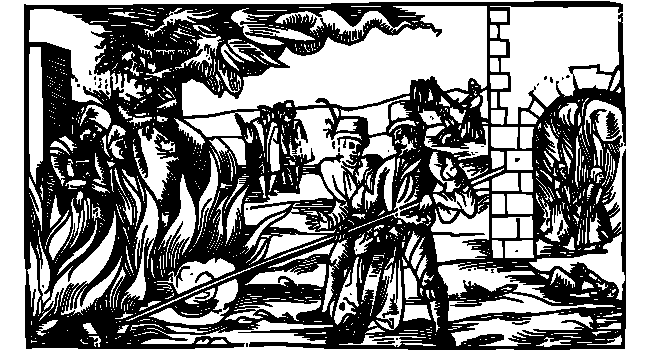
\includegraphics[width=\textwidth]{./images/religion04.pdf}
    % \caption{Inline Example Image}
\end{figure}

\subsection{\textbf{Religious Roles}}

The "Religious Roles" field represents the various positions and titles within a fictional religious organization or belief system. These roles range from leaders and spiritual advisors, to assistants and messengers, to protectors and mediators. Each role comes with its own set of responsibilities and privileges, reflecting the unique aspects and beliefs of the religion it represents. Some religious roles may be highly respected and hold significant power within the community, while others may be more solitary or focused on specific tasks. This field is important for creating well-rounded and diverse religious systems within the game world, and for providing players with the opportunity to explore different aspects of spirituality and faith. Whether a player chooses to play a charismatic leader or a solitary mystic, the "Religious Roles" field offers a wealth of opportunities for role-playing and character development.

\begin{enumerate}
    \item \textbf{Abbot/Abbess:} The leader of a monastery or convent.
    \item \textbf{Archbishop:} A bishop who oversees multiple dioceses.
    \item \textbf{Acolyte:} An assistant or beginner in religious service.
    \item \textbf{Bishop:} An overseer of a specific area or diocese within a church.
    \item \textbf{Chaplain:} A spiritual advisor in a specific setting, such as a hospital or military unit.
    \item \textbf{Cult Leader:} Usually a charismatic head of a small group of highly devoted followers.
    \item \textbf{Disciple:} A dedicated follower of a religious teacher or leader.
    \item \textbf{Elder:} An experienced and respected member of a religious community.
    \item \textbf{Evangelist:} A religious figure who spreads the gospel or message of their faith to others.
    \item \textbf{Guru:} A spiritual teacher.
    \item \textbf{Inquisitor:} An official tasked with finding and "correcting" people who have broken religious rules.
    \item \textbf{Martyr:} A person who dies for their religious beliefs.
    \item \textbf{Missionary:} Dedicated to converting others, usually in distant geographic areas.
    \item \textbf{Monk/Nun:} Belongs to a monastery or convent.
    \item \textbf{Mystic:} A person who has direct experience of ultimate reality through spiritual or mystical practices.
    \item \textbf{Patriarch/Matriarch:} The leader of an organized religion.
    \item \textbf{Pilgrim:} One traveling to a holy site or landmark.
    \item \textbf{Priest/Priestess:} Someone authorized to administer sacraments as an ordained member of a church.
    \item \textbf{Prophet:} One inspired to utter revelations or predictions, often in service to a deity.
    \item \textbf{Reverend:} An honorific title given to a religious figure.
    \item \textbf{Sacred Courtesan:} Has sex, often with strangers, in service to a religion and for a symbolic price.
    \item \textbf{Mediator:} A person who helps resolve conflicts and bring people together through spiritual means.
    \item \textbf{Seeker:} One who is searching for spiritual knowledge and understanding.
    \item \textbf{Temple Guardian:} A protector of a religious site, such as a temple or shrine.
    \item \textbf{Wandering Monk:} A roving spiritual teacher who travels from place to place, spreading religious teachings.
    \item \textbf{Witch:} A practitioner of magic who uses their powers for spiritual purposes.
    \item \textbf{Healer:} A person skilled in the use of herbs, prayers, or other methods to cure illnesses and injuries.
    \item \textbf{Oracle:} A person or entity that provides insight or prophesies into the future or hidden knowledge.
    \item \textbf{Seer:} A person who has the ability to see and understand things that others cannot, often through spiritual means.
    \item \textbf{Divine Herald:} A messenger of the gods, responsible for delivering messages and performing sacred duties.
    \item \textbf{Sanctuary Keeper:} The caretaker of a sacred place, responsible for maintaining its sanctity and protecting it.
    \item \textbf{Temple Guardian:} A protector of a religious site, such as a temple or shrine.
    \item \textbf{Shrine Maiden:} A female spiritual attendant, responsible for maintaining the purity and sanctity of a shrine.
    \item \textbf{Ritualist:} A person skilled in the performance of religious rituals and ceremonies.
    \item \textbf{Visionary:} A person who receives and interprets divine visions and messages.
    \item \textbf{Soothsayer:} A person who predicts future events based on astrology, dreams, or other forms of divination.
    \item \textbf{Holy Knight:} A warrior who serves a religious cause and protects the faithful.
    \item \textbf{Chant Master:} A person who leads religious music and song, often in a religious setting.
    \item \textbf{Deacon:} A clergy member responsible for serving the needs of a congregation.
    \item \textbf{Minister:} A religious leader who serves a specific denomination or congregation.
    \item \textbf{Deity:} A supernatural being worshipped as having power over the world and human affairs.
    \item \textbf{Saint:} A person recognized as holy or virtuous by a particular religion.
    \item \textbf{Apostle:} A messenger or disciple of a religious teacher or leader.
    \item \textbf{Recluse:} One who lives in solitude for spiritual or religious reasons.
    \item \textbf{Necromancer:} A person who communicates with the dead for the purpose of gaining knowledge or guidance.
\end{enumerate}

\begin{figure}[h]
    \centering
    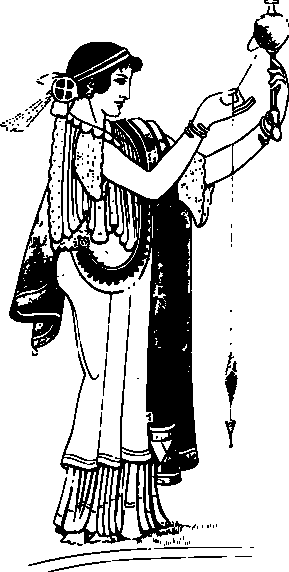
\includegraphics[width=\textwidth]{./images/religion02.pdf}
    % \caption{Inline Example Image}
\end{figure}

\subsection{\textbf{Practices/Rituals}}

The "Practices/Rituals" field is an important aspect of a character's spiritual profile, as it allows players to flesh out their character's religious beliefs and observances. This field covers the specific rituals or practices that the character engages in, such as daily prayers or meditations, monthly celebrations or ceremonies, seasonal rituals, or life milestones. In addition to the type of ritual, this field may also include information on the frequency, location, and details of the ritual itself. For example, a character might participate in a monthly full moon ritual that involves offering incense, reciting prayers, and communing with their deity or spirit guide. By including this information, players can help to create a more vivid and immersive representation of their character's spirituality. Additionally, this information can also be used to drive roleplaying decisions, such as the character's reactions to certain situations or interactions with others. Overall, the "Practices/Rituals" field is a valuable tool for creating well-rounded, believable characters with unique spiritual perspectives.

\begin{enumerate}

    \item \textbf{Daily prayers or meditations:}
    This entry would describe any daily spiritual practices the character engages in, such as daily prayers, meditations, or affirmations. The player could specify the frequency, duration, and location of these activities, as well as the purpose or intention behind them.
    
    \item \textbf{Monthly religious celebrations or ceremonies:}
    This entry would describe any monthly religious events or observances the character participates in, such as full moon rituals, holy days, or feast days. The player could detail the specific celebrations or ceremonies, the significance or meaning behind them, and the role the character plays in these events.

    \begin{center}
        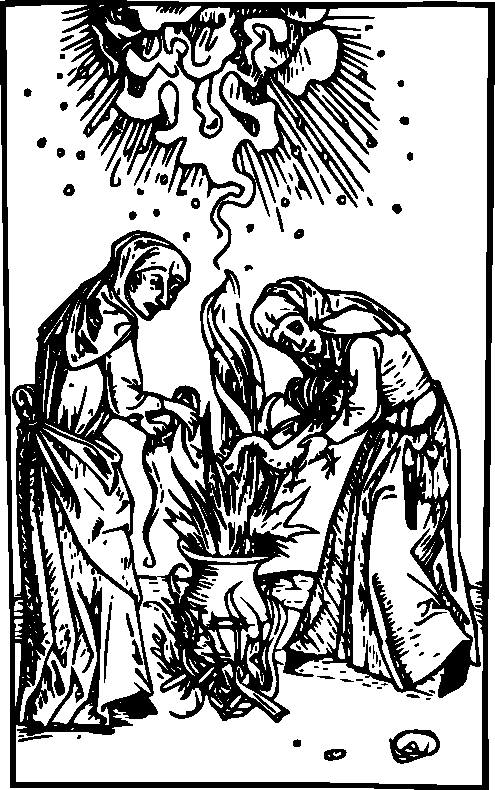
\includegraphics[width=0.6\textwidth]{./images/religion07.pdf}
    \end{center}
    
    \item \textbf{Seasonal rituals or observances:}
    This entry would describe any seasonal spiritual practices or events the character participates in, such as solstice or equinox ceremonies, harvest festivals, or other events that mark the changing of the seasons. The player could detail the specific rituals or observances, the significance or meaning behind them, and the role the character plays in these events.
    
    \item \textbf{Life milestones or rites of passage:}
    This entry would describe any spiritual practices or events that mark important transitions or milestones in the character's life, such as birth, adolescence, marriage, or death. The player could detail the specific rituals or observances, the significance or meaning behind them, and the role the character plays in these events.

    \item \textbf{Fasting or dietary restrictions:}
    This entry would describe any dietary restrictions or fasting practices the character engages in for religious or spiritual reasons. The player could specify the type of fasting, the frequency, and the reason behind it, as well as any specific dietary restrictions the character follows, such as vegetarianism or prohibitions against certain foods or ingredients.
    
    \item \textbf{Pilgrimages or sacred journeys:}
    This entry would describe any pilgrimages or sacred journeys the character has taken or plans to take, such as visiting holy sites, participating in spiritual retreats, or making offerings at shrines or temples. The player could detail the specific destinations, the significance or meaning behind these journeys, and any preparations or rituals involved in making these trips.

    \item \textbf{Animal or human sacrifices:}
    This entry would describe any instances where the character participates in or witnesses animal or human sacrifices as part of their religious or spiritual beliefs. The player could detail the specific reasons for these sacrifices, the religious or spiritual significance behind them, and any emotional or ethical conflicts the character experiences in relation to these practices.

    \item \textbf{Chanting, Singing, or Dancing:}
    These rituals often involve repetitive vocalizations or movements that are meant to connect the individual with the divine or the spiritual realm. In some religions, singing and dancing are also used to tell religious stories or to give praise to a deity. These practices can be performed individually or as part of a group, and they can take place in a designated religious space or in everyday life.

    \item \textbf{Use of Religious Symbols or Artifacts:}
    Religious symbols and artifacts can hold a significant spiritual meaning for an individual and can be used in religious practices and rituals. They may include objects such as crosses, statues, altars, prayer beads, or other items that are used to focus the individual's thoughts and emotions towards their religion. The use of these symbols and artifacts may also serve as a way to connect the individual with the divine, to protect themselves from harm, or to mark special moments in their spiritual journey.
    
    \item \textbf{Spiritual or Physical Purification Rituals:}
    Purification rituals can take many forms and serve different purposes, but they typically aim to cleanse the individual of negative energies or influences. These rituals may involve washing or bathing, fasting, meditation, or the use of special incense or herbs. In some cultures, spiritual purification may be seen as a necessary step before engaging in other religious practices or before coming into contact with sacred spaces or objects.
    
    \item \textbf{Offering of Incense or Candles:}
    The burning of incense or candles is a common religious practice in many cultures and can serve a variety of purposes. It may be used to create a peaceful or meditative atmosphere, to communicate with the divine, to make offerings to a deity, or to symbolize the individual's devotion. The act of lighting incense or candles may also involve specific rituals or prayers, making the act of offering a spiritual or sacred act.
    
    \item \textbf{Recitation of Prayers, Mantras, or Affirmations:}
    The recitation of prayers, mantras, or affirmations is a common practice in many religions and spiritual traditions. These verbal expressions can serve as a way to connect with the divine, to focus the individual's thoughts, or to give praise or gratitude. Prayers and mantras may be recited individually or in a group, and they may involve specific actions such as bowing, kneeling, or making offerings.
    
    \item \textbf{Meditation or Visualization Exercises:}
    Meditation and visualization exercises are commonly used in spiritual and religious contexts as a way to focus the mind and connect with the divine. These practices can involve focusing on a specific image or thought, repeating a mantra or affirmation, or simply letting the mind become still. Meditation and visualization can be performed in a quiet or sacred space, or as part of a larger ritual or ceremony.

    \item \textbf{Communication with Gods, Spirits, or Ancestors:}
    Many spiritual and religious traditions involve communicating with gods, spirits, or ancestors as a way to seek guidance, protection, or to make offerings. This communication can take many forms, including prayer, divination, or mediumship. In some cultures, communication with the spiritual realm is seen as a necessary part of daily life, while in others it is reserved for special occasions or life events.

    \item \textbf{Divination or prophetic rituals:}
    Divination or prophetic rituals involve seeking insight or knowledge of the future, or receiving guidance from a higher power. This could include practices like tarot readings, casting bones, or interpreting omens. These rituals are often performed by a designated individual within the religious community, such as a priest or shaman.
    
    \item \textbf{Healing or protection rituals:}
    Healing or protection rituals are performed with the intention of restoring health or providing protection to an individual or community. These could include practices like laying on of hands, reciting incantations, or using magical symbols. These rituals may be performed by a religious leader or by individuals seeking to heal themselves or others.

    \item \textbf{Rituals involving the use of psychoactive substances:}
    Rituals involving the use of psychoactive substances, such as entheogenic plants or psychedelics, are sometimes used in religious or spiritual practices. These substances are believed to alter the state of consciousness, allowing the individual to connect with the divine or access higher states of awareness. These practices are often performed under the guidance of a shaman or spiritual leader and are considered sacred within some religious traditions.

    \item \textbf{Group meditation or prayer sessions:}
    Group meditation or prayer sessions involve a community of individuals coming together to meditate, pray, or perform other spiritual practices in unison. These sessions are often led by a religious leader or facilitator and may be performed on a regular basis, such as daily or weekly. Group meditation or prayer sessions can provide a sense of community and support for those involved and can also help to deepen individual spiritual experiences.
    
    \item \textbf{Choral performances or religious music:}
    Choral performances or religious music involve singing or playing musical instruments in a religious or spiritual context. This could include hymns, chants, or gospel songs. These performances may be performed by a choir.
    
\end{enumerate}

\end{document}



% \begin{figure}[h]
%     \centering
%     \includegraphics[width=\textwidth]{./images/personality05.pdf}
%     % \caption{Inline Example Image}
% \end{figure}
